
\documentclass[8pt]{beamer}

\usepackage[german]{babel}
\usepackage[utf8]{inputenc}
\usepackage{pdfpages}
\usepackage{color}
\usepackage{graphicx, import}
\usepackage{amsmath}
\usepackage{amssymb}
\usepackage{physics} % norm
\usepackage{tikz}
\usepackage{tkz-euclide}
%\usepackage{enumitem}
\usepackage{pgfplots}
\usepackage{multicol}
\usepackage{tabularx}
\usepackage[numbers, square]{natbib}
\usepackage{mathtools}
\usepackage{transparent}
\usepackage{caption} % change style of figure 
\usepackage{subcaption}
\usepackage{csquotes} % automatic left quotation marks
\usepackage{booktabs}
\usepackage[]{algorithm2e}
\usepackage[super]{nth}
\usepackage{autonum} % auto equation numbering
\usepackage{bbm}
\usepackage{scalerel,stackengine}
\usepackage{mdframed}
\usepackage{array}

\captionsetup*[subfigure]{position=bottom}

\MakeOuterQuote{"}

\usetikzlibrary{calc, positioning,backgrounds, fit, patterns,shapes, snakes, chains, arrows, decorations.markings, arrows.meta}
%\tikzexternalize[prefix=out/figures/]
\newcolumntype{Y}{>{\centering\arraybackslash}X} % centered equidistant columns
\newcolumntype{R}[1]{>{\PreserveBackslash\raggedleft}p{#1}}
\newcolumntype{L}[1]{>{\PreserveBackslash\raggedright}p{#1}}

\bibliographystyle{plainnat}
\usetheme[block=transparent]{metropolis}
\usecolortheme{orchid}
\setbeamercolor{block body}{use=structure,fg=structure.fg,bg=structure.bg}
\setbeamercolor{block title}{use=structure,fg=structure.fg,bg=structure.bg}
\setbeamertemplate{frame footer}{\insertshortauthor\hfill\insertshortinstitute}
\setbeamercolor{footline}{fg=gray}

\DeclarePairedDelimiterX{\infdiv}[2]{(}{)}{%
	#1\;\delimsize\|\;#2%
}

\renewcommand{\epsilon}{\varepsilon}

\DeclareMathOperator*{\argmax}{arg\,max}
\DeclareMathOperator*{\argmin}{arg\,min}
\DeclareMathOperator{\JSD}{JS}
\DeclareMathOperator{\KL}{KL}
\newcommand{\T}{\mathrm{T}}
\newcommand{\R}{\mathbb{R}}
\newcommand{\cX}{\mathcal{X}}
\newcommand{\cG}{\mathcal{G}}
\newcommand{\cD}{\mathcal{D}}
\newcommand{\cF}{\mathcal{F}}
\newcommand{\cO}{\mathcal{O}}
\newcommand{\cZ}{\mathcal{Z}}
\newcommand{\cB}{\mathcal{B}}
\newcommand{\N}{\mathbb{N}}
\newcommand{\E}{\mathbb{E}}
\newcommand{\Z}{\mathbb{Z}}
\newcommand{\fL}{\mathfrak{L}}
\newcommand{\RL}{\textsc{RingLoading}\xspace}
\newcommand{\RRL}{\textsc{RRL}\xspace}
\newcommand{\RRLWC}{\textsc{RRLwC}\xspace}
\newcommand{\dOne}{\mathbbm{1}}
\newcommand{\Lopt}{L^{\mathrm{opt}}}

\newcommand\equalhat{\mathrel{\stackon[1.5pt]{=}{\stretchto{%
				\scalerel*[\widthof{=}]{\wedge}{\rule{1ex}{3ex}}}{0.5ex}}}}

\makeatletter
\DeclareRobustCommand\onedot{\futurelet\@let@token\@onedot}
\def\@onedot{\ifx\@let@token.\else.\null\fi\xspace}

\def\eg{\emph{e.g}\onedot} \def\Eg{\emph{E.g}\onedot}
\def\ie{\emph{i.e}\onedot} \def\Ie{\emph{I.e}\onedot}
\def\cf{\emph{c.f}\onedot} \def\Cf{\emph{C.f}\onedot}
\def\etc{\emph{etc}\onedot} \def\vs{\emph{vs}\onedot}
\def\iid{\emph{i.i.d}\onedot} \def \Iid{\emph{I.i.d}\onedot}
\def\wrt{w.r.t\onedot} \def\dof{d.o.f\onedot}
\def\etal{\emph{et al}\onedot}
\makeatother


\makeatletter
\def\th@claim{%
	\normalfont % body font
	\setbeamercolor{block title example}{bg=red!65!black,fg=structure.bg}
	\setbeamercolor{block body example}{bg=red!80!black!20,fg=black}
	\setbeamercolor{example text}{fg=red}
	\def\inserttheoremblockenv{exampleblock}
}
\makeatother
\theoremstyle{claim}
\newtheorem{mytheorem}[theorem]{Theorem}
\newtheorem{mylemma}[theorem]{Lemma}
\newtheorem{mycorollary}[theorem]{Korollar}

%\theoremstyle{theorem}
%\newtheorem{lemma}[definition]{Lemma}
%\newtheorem{corollary}[definition]{Corollary}
%\newtheorem{remark}[definition]{Remark}
%\newtheorem{proposition}[definition]{Proposition}
%\theoremstyle{break}
%\newtheorem{theorem}[definition]{Theorem}
%\newtheorem{condition}[definition]{Condition}
\setbeamertemplate{section in toc}[sections numbered]
\setbeamertemplate{subsection in toc}{\leavevmode\leftskip=3.2em\rlap{\hskip-2em\inserttocsectionnumber.\inserttocsubsectionnumber}\inserttocsubsection\par}
\setbeamercolor{section in toc}{fg=black}
\setbeamercolor{subsection in toc}{fg=black}
\setbeamercolor{toc}{fg=black}

\AtBeginSection[]{}

\title[]{Das Ring Loading Problem}
%\subtitle{Seminar \glqq Mathematische Aspekte des maschinellen Lernens\grqq}
\author[Nikolas Klug]{Nikolas Klug}
\institute[Universität Augsburg]{Universität Augsburg}
\date{23. Dezember 2021}


\begin{document}
	{
	\setbeamertemplate{footline}{}
	\begin{frame}
		\titlepage
	\end{frame}
	}
	\addtocounter{framenumber}{-1}

	\begin{frame}{Hauptquelle}
%		\begin{NoHyper}
%			\tableofcontents[]
%		\end{NoHyper}

		\emph{The Ring Loading Problem},\\
		 Alexander Schrijver, Paul Seymour, Peter Winkler, \\
		 \emph{SIAM Review 41 (4), 1999.}\\
	\end{frame}
	
	\begin{frame}{Problemstellung}
		Das Ring Loading Problem tritt bei der Planung von SONET Ringen auf.
		\vspace{1mm}
		\begin{center}
		\begin{tikzpicture}[font=\large, node/.style={circle,thick,draw},scale=0.8, transform shape]
			\foreach \a in {1,2,...,6}{
				\draw (\a*360/6: 3cm) node[] (\a) {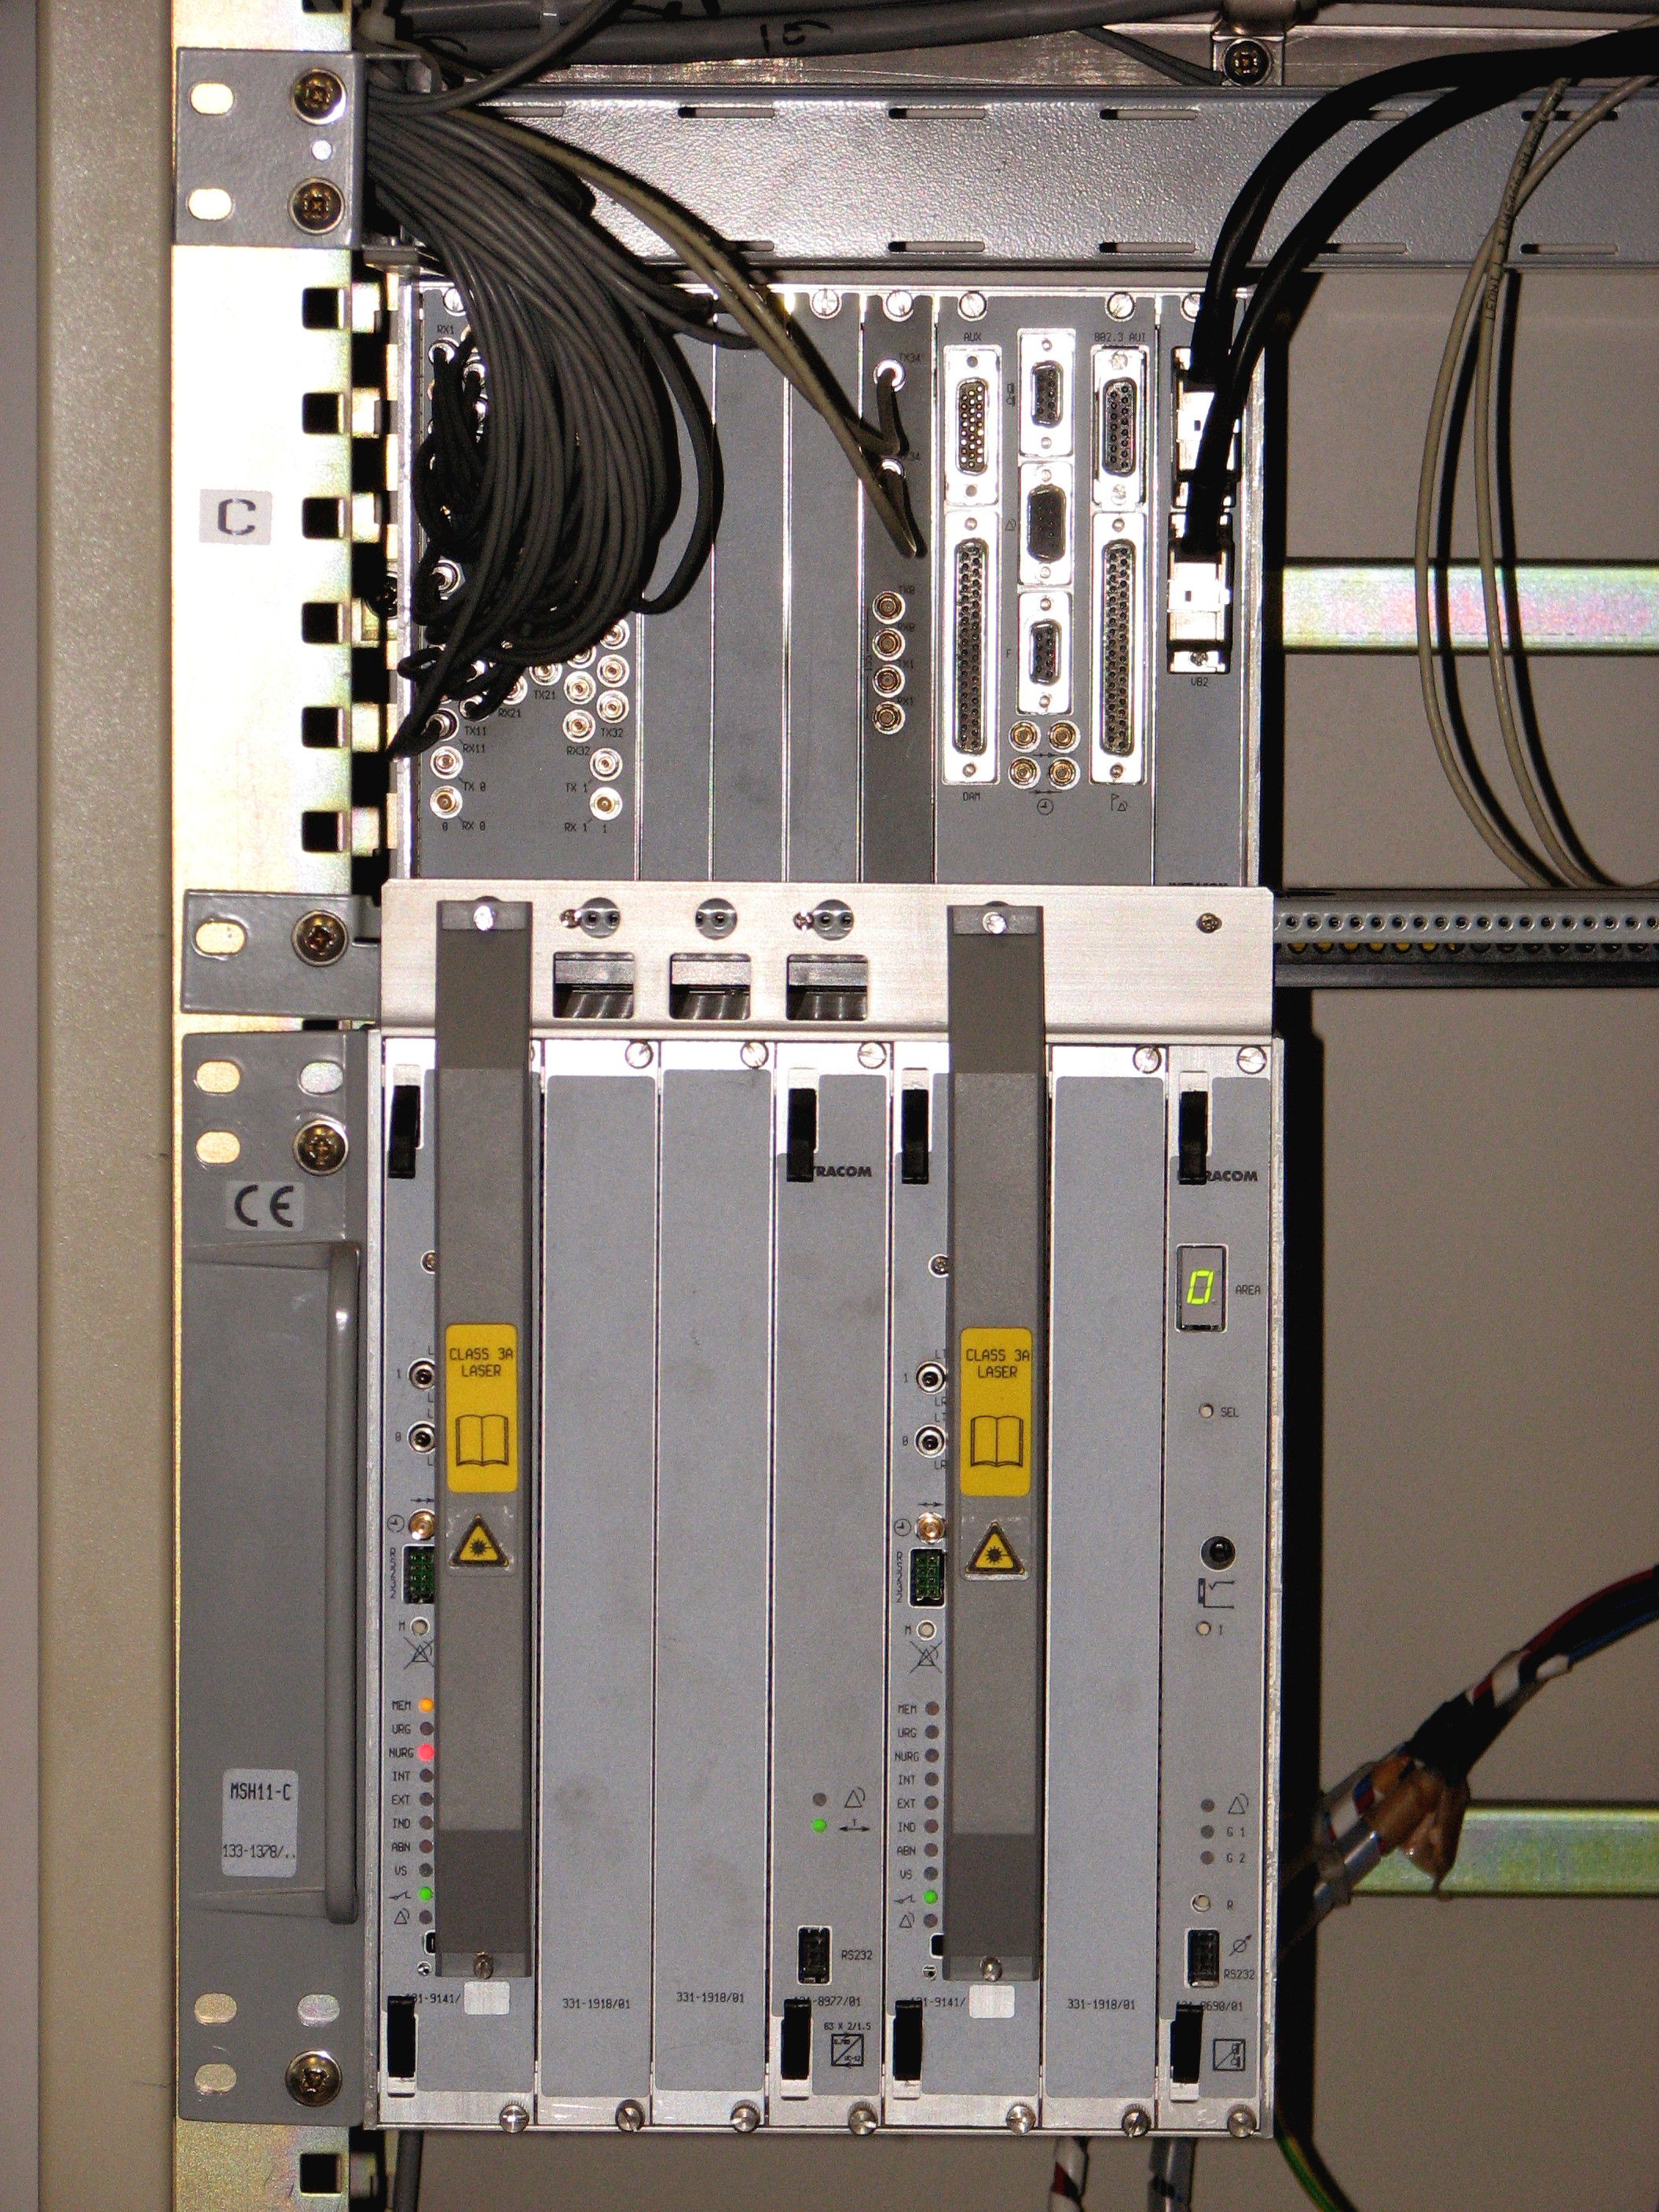
\includegraphics[scale=0.01]{figures/adm.jpg}};
			}
			\foreach \a [count=\x from 2]in {1,2,...,5}{
				\path[color=black, line width=0.25mm](\a) edge node[pos=0.8,above=-1mm, sloped,gray]{} (\x) {};	
			}
			\draw[color=black, line width=0.25mm](6) edge (1) {};	
			\path[->, color=black, line width=1pt](-4, 2)edge(2);
			\node (a) at (-5, 1.7) {Add-Drop Multiplexer};
			\path[->, color=black, line width=1pt](4, -2) edge(-30:2.8);
			\node (a) at (5, -2.3) {Glasfaserkabel};
			\path[color=black](1) edge  (60:4.5cm) {};	
			\path[color=black](2) edge  (120:4.5cm) {};	
			\path[color=black](3) edge  (180:4.5cm) {};
			\path[color=black](4) edge  (240:4.5cm) {};
			\path[color=black](5) edge  (300:4.5cm) {};
			\path[color=black](6) edge  (0:4.5cm) {};			
			\node[] at (-6, 0) {};
			\node[] at (6, 0) {};
		\end{tikzpicture}
	\end{center}
	\vskip0pt plus 1filll
	\scriptsize{ADM Abbildung von I, Adamantios, CC BY-SA 3.0, https://commons.wikimedia.org/w/index.php?curid=2432326}
	\end{frame}

	\section{Formalisierung}
	
	\begin{frame}{Formalisierung}
		\begin{columns}
			\column{0.6\linewidth}
			Ring $\equalhat$ Graph mit $n$ Knoten.\\
			Knotenmenge $V = [n] = \{1, 2, 3, \dots, n\}$.\\
			Kantenmenge $E = \{\{k, k+1\}\ |\ k \in [n]\}$\\
			~\\\pause
			Für jedes Paar von Knoten $i, j \in [n], i < j$: \emph{Nachfrage} (engl. demand) $d_{i, j} \in \R_{\geq 0}$.\\
			~\\\pause
			$d_{i,j}$ wird \emph{vorwärts} gerouted, falls die Kante $\{n, 1\}$ nicht genutzt wird.\\
			Sonst wird $d_{i,j}$ \emph{rückwärts} gerouted.
			\column{0.4\linewidth}
			\centering
\begin{tikzpicture}[font=\scriptsize, node/.style={circle,thick,draw},
	l_2/.style={line width =0.25mm},
	scale=0.9, transform shape]
	\draw[l_2] (2,0) arc (0:360:2);	
	% equidistant points and arc
	\foreach \x [count=\p] in {0,...,7} {
		\node[shape=circle,fill=black, scale=0.5] (\p) at (\x*45-135:2) {};
	};
	\foreach \x [count=\p] in {0,...,7} {
		\draw (225 + \x*45:1.7) node {\p};
		%				\draw (-30-\x*60:2.4) node {$\bar{\p}$};
	}; 
%	\node (bottom) at (0, -2.8) {};
\end{tikzpicture}

		\end{columns} 
	\end{frame}
	
	\begin{frame}{Routings und Lasten}
		\begin{columns}
			\column{0.6\linewidth}
			\begin{definition}[Routing]
			\label{def:routing}
			Ein \emph{reellwertiges Routing} in einem Ring der Größe $n \in \N$ ist eine Funktion
			\begin{equation}
				\Phi: \{(i, j)\ |\ i, j \in [n], i < j \} \rightarrow [0, 1] \ .
				\end{equation}
				Ein \emph{binäres Routing} ist ein reellwertiges Routing $\Phi$, das nur Werte in $\{0, 1\}$ annimmt. 
			\end{definition}\pause		
			\begin{definition}[Kantenlast, Ringlast]
				\label{def:edge-load}
				Sei $\Phi$ ein Routing.
				Für jede Kante $\{k, k+1\}$, $k \in [n]$, definieren wir die \emph{Kantenlast} $L_k(\Phi)$ als:
				\begin{equation}
					\label{eq:edge-load}
					L_k(\Phi) \coloneqq \sum_{\substack{1 \leq i < j \leq n,\\ k \in [i, j)}} d_{i, j} \Phi(i, j) + \sum_{\substack{1 \leq i < j \leq n,\\ k \notin [i, j)}} d_{i, j} (1 - \Phi(i, j)) \ .
				\end{equation}
				Die \emph{Ringlast} $L(\Phi)$ ist die maximale Kantenlast des Routings $\Phi$.
			\end{definition}
			\column{0.4\linewidth}
			\centering
\begin{tikzpicture}[font=\scriptsize, node/.style={circle,thick,draw},
	l_2/.style={line width =0.25mm},
	scale=0.9, transform shape]
	\draw[l_2] (2,0) arc (0:360:2);	
	% equidistant points and arc
	\foreach \x [count=\p] in {0,...,7} {
		\node[shape=circle,fill=black, scale=0.5] (\p) at (\x*45-135:2) {};
	};
	\foreach \x [count=\p] in {0,...,7} {
		\draw (225 + \x*45:1.7) node {\p};
		%				\draw (-30-\x*60:2.4) node {$\bar{\p}$};
	}; 
%	\node (bottom) at (0, -2.8) {};
\end{tikzpicture}

		\end{columns} 
	\end{frame}

	\begin{frame}{Das Ring Loading Problem}
		\begin{center}
			\begin{mdframed}
				\centering
				\textsc{RingLoading}\\[0.7em]
				\begin{tabularx}{\textwidth}{rl}
					{\bfseries Eingabe}: & Ringgröße $n \in \N$, und Nachfragen $d_{i, j} \in \R_{\geq 0}$ für alle $1 \leq i<j\leq n$.\\
					{\bfseries Ausgabe}: & Binäres Routing $\Phi$, welches $L(\Phi) = \max_{i \in [n]} L_i(\Phi)$ minimiert.
				\end{tabularx}
			\end{mdframed}
		\end{center}\pause
		Instanzgröße: $\cO(K \log D + \log n)$, wobei $D$ maximale Nachfrage und $K$ Anzahl nicht-negativer Nachfragen.
	\end{frame}

	\begin{frame}{NP-Vollständigkeit}
		\RL als Entscheidungsproblem:
		\begin{quote}
			"Gegeben eine \RL Instanz und $T \in \N$, existiert ein binäres Routing $\Phi$ mit Ringlast $L(\Phi) \leq T$?"
		\end{quote}\pause
		\begin{mytheorem}
			\RL als Entscheidungsproblem ist NP-vollständig.
		\end{mytheorem}\pause
		\begin{proof}\let\qed\relax
			\underline{\RL liegt in NP:} Routing ist Zertifikat der Größe $\cO(K)$\\\pause
			\underline{NP-Vollständigkeit:}\\
			Wir reduzieren \textsc{PARTITION}.
		    Eine Instanz $J$ besteht aus $m$ natürlichen Zahlen $z_1, \ldots, z_m \in \N$.\\
		    Frage: Existiert eine Menge $S \subseteq [m]$, sodass:
			\begin{equation}
				\sum_{i \in S} z_i = \frac{1}{2} \sum_{i \in [m]} z_i = \sum_{j \in [m] \setminus S} z_j\ .
			\end{equation}
		\end{proof}
	\end{frame}

	\begin{frame}
		\begin{columns}
		\column{0.55\linewidth}
		Wir konstruieren die folgende \RL Instanz:
		\centering
		\begin{tikzpicture}[font=\scriptsize, node/.style={circle,thick,draw},
			l_2/.style={line width =0.25mm},
			scale=1, transform shape]
			% equidistant points and arc
			\foreach \x [count=\p] in {0,...,7} {
				\node[shape=circle,fill=black, scale=0.5] (\p) at (\x*45-135:2) {};
			};
			\foreach \x [count=\p] in {0,...,3} {
				\draw (225 + \x*45:1.7) node {\p};
				%				\draw (-30-\x*60:2.4) node {$\bar{\p}$};
			}; 
			\draw (225 + 4*45:1.7) node {$m$};
			\draw (225 + 5*45:1.7) node {$m+1$};
			\draw (225 + 6*45:1.6) node {$m+2$};
			\draw (225 + 7*45:1.45) node {$m+3$};
			
			\draw[l_2] (5) arc (45:360:2);
			\draw[line width =1.3pt, line cap=round, dash pattern=on 0pt off 10pt] (12:2) arc(12:35:2);
			
			
			\draw[<->] (1)  to [out=157.5,in=-90] (180:2.5) to [out=90,in=-170](7);
			\draw[<->] (2)  to [out=-157.5,in=-67.5] (-157.5:2.8) to [out=112.5,in=-180] (7);
			\draw[<->] (3)  to [out=-112.5,in=-45] (-135:3.2) to [out=135,in=-190] (7);
			\draw[<->] (4)  to [out=67.5,in=-22.5] (67.5:3) to [out=157.5,in=100] (7);
			\draw[<->] (5)  to [out=112.5,in=0] (90:2.7) to [out=180,in=85] (7);
			
			\draw[<->] (6)  to [out=160,in=22.5] (112.5:2.2) to [out=-157.5,in=60] (7);
			\draw[<->] (8)  to [out=100,in=-135] (150:2.2) to [out=45,in=-155] (7);
			
			\node (a) at (-142:2.3) {$z_1$};
			\node (b) at (-105:2.45) {$z_2$};
			\node (c) at (-85:2.8) {$z_3$};
			\node (d) at (45:3.1) {$z_4$};
			\node (e) at (58:2.5) {$z_m$};
			\node (d) at (95:2.3) {$\frac{T}{2}$};
			\node (f) at (175:2.2) {$\frac{T}{2}$};
			
			\node (left) at (-3, 0) {};
			\node (right) at (3, 0) {};
			%		\draw[dashed] (1) -- (3) -- (5) -- (1);
			% axes
			%		\draw [dotted, gray] (-2.6,0) -- (2.6,0);
			%		\draw [dotted, gray] (0,-2.15) -- (0,2.15);
		\end{tikzpicture}\\
		wobei $T =\sum_{i \in [m]} z_i$.\\\pause
		\column{.45\linewidth}
		Sei $A \subseteq [m]$ Lösung von \textsc{Partition}.
		Wir wählen
		\begin{align}
			\Phi(i, m+2) &= 1 \quad \forall i \in A \\
			\Phi(i, m+2) &= 0 \quad \forall i \in [m] \setminus A \\
			\Phi(m+1, m+2) & = \Phi(m+2, m+3) = 1 \ .
		\end{align}\pause
		
		Sei $\Phi$ Lösung der \RL Instanz.
		Dann löst
		\begin{equation}
			A' \coloneqq \{i \ |\ i \in [m] \text{ and } \Phi(i, m+2) = 1\}
		\end{equation}
		die \textsc{Partition} Instanz.
		\qed
	\end{columns}
	\end{frame}

	\begin{frame}{Relaxed Ring Loading}
		Für den Approximationsalgorithmus lösen wir zunächst folgendes Problem:
		\vspace{5mm}
		\begin{center}
			\begin{mdframed}
				\centering
				\textsc{RelaxedRingLoading} (\textsc{RRL})\\[0.7em]
				\begin{tabular}{rl}
					{\bfseries Eingabe}: & Ringgröße $n \in \N$, und Nachfragen $d_{i, j} \in \R_{\geq 0}$ für alle $1 \leq i<j\leq n$.\\
					{\bfseries Ausgabe}: & Reellwertiges Routing $\Phi$, welches $L(\Phi) = \max_{i \in [n]} L_i(\Phi)$ minimiert.
				\end{tabular}
			\end{mdframed}
		\end{center}
	\end{frame}
	
	
	\begin{frame}{Idee des Approximationsalgorithmus}
		Sei $I$ eine \RL Instanz.
		\begin{enumerate}
			\item[1.] Bestimme Lösung des relaxierten Problems, in der möglichst wenige Nachfragen aufgeteilt werden.
			\item[2.] Route die aufgeteilten Nachfragen so um, dass sich die Ringlast möglichst wenig erhöht.
		\end{enumerate}
	\end{frame}

	\begin{frame}{Minimale Lösungen}
		\begin{definition}
			Sei $\Phi^\ast$ eine Optimallösung einer \RRL Instanz.
			$\Phi^\ast$ heißt \emph{minimal}, falls \emph{kein} anderes optimales Routing $\Phi'$ existiert, sodass:
			\begin{align}
				L_i(\Phi') &\leq L_i(\Phi^\ast) \quad \text{ für alle } i \in [n] \ ,\\
				L_j(\Phi') &< L_j(\Phi^\ast) \quad \text{ für mindestens ein } j \in [n] \ .
			\end{align}
		\end{definition}\pause
		\begin{mytheorem}
			Sei $\Phi^\ast$ eine Minimallösung einer \RRL Instanz der Größe $n$.
			Dann werden in $\Phi^\ast$ höchstens $\lfloor \frac{n}{2} \rfloor$ Nachfragen aufgeteilt.
		\end{mytheorem}
	\end{frame}

	\begin{frame}{Parallele und schneidende Nachfragen}
		\begin{columns}
		\column{0.6\linewidth}
		\begin{definition}
			Seien $i, j, u, v \in [n]$, $i < j, u < v$ und $d_{i,j}, d_{u, v}$ zwei Nachfragen.
			\begin{itemize}
				\item<1-> $d_{i, j}$ und $d_{u, v}$ \emph{schneiden sich}, falls $i, j, u, v$ paarweise verschieden sind und $i < u < j < h$ oder $u < i < h < j$.
				\item<2-> $d_{i, j}$ und $d_{u, v}$ sind \emph{parallel}, falls sie sich nicht schneiden.
				\item<3-> Seien $d_{i, j}$ und $d_{u, v}$ parallel und $j < v$.
				Die Kante $\{k, k+1\}$ liegt \emph{zwischen} $d_{i,j}$ und $d_{u, v}$, falls sie auf der vorderen Route von genau einer der Nachfragen liegt (falls $i \geq u$) oder falls sie auf der hinteren Route beider Nachfragen liegt (falls $j \leq u$).
			\end{itemize}
		\end{definition}
		\column{0.4\linewidth}
		\visible<1->{\centering
\begin{tikzpicture}[font=\scriptsize, node/.style={circle,thick,draw},
	l_2/.style={line width =0.25mm},
	scale=0.9, transform shape]
	\draw[l_2] (2,0) arc (0:360:2);	
	% equidistant points and arc
	\foreach \x [count=\p] in {0,...,7} {
		\node[shape=circle,fill=black, scale=0.5] (\p) at (\x*45-135:2) {};
	};
	\foreach \x [count=\p] in {0,...,7} {
		\draw (225 + \x*45:1.7) node {\p};
		%				\draw (-30-\x*60:2.4) node {$\bar{\p}$};
	}; 
%	\node (bottom) at (0, -2.8) {};
\end{tikzpicture}
}
		\end{columns}
	\end{frame}

	\begin{frame}
		\begin{mylemma}
			Sei $\Phi^\ast$ ein minimales Routing und $d_{i, j}$, $d_{u, v}$ parallele Nachfragen.
			Dann werden durch keine der Kanten zwischen $d_{i, j}$ und $d_{u, v}$ beide Nachfragen gerouted.
		\end{mylemma}
		\vspace{5mm}
		\begin{proof}[Beweisskizze.]\let\qed\relax
			Seien $d_{i, j}$ und $d_{u, v}$ zwei Nachfragen, $\{k, k+1\}$ eine Kante zwischen $d_{i, j}$ und $d_{g, h}$.
			Seien $\alpha, \beta$ die Anteile, die durch $\{k, k+1\}$ gerouted werden und o.B.d.A. $\alpha < \beta$.
		\end{proof}
		\begin{center}
			\begin{minipage}{0.4\linewidth}
					\centering
\begin{tikzpicture}[font=\scriptsize, node/.style={circle,thick,draw},
	l_2/.style={line width =0.25mm},
	scale=0.9, transform shape]
	\draw[l_2] (2,0) arc (0:360:2);	
	% equidistant points and arc
	\foreach \x [count=\p] in {0,...,7} {
		\node[shape=circle,fill=black, scale=0.5] (\p) at (\x*45-135:2) {};
	};
	\foreach \x [count=\p] in {0,...,7} {
		\draw (225 + \x*45:1.7) node {\p};
		%				\draw (-30-\x*60:2.4) node {$\bar{\p}$};
	}; 
%	\node (bottom) at (0, -2.8) {};
\end{tikzpicture}

			\end{minipage}
			\hspace{1.3cm}
			\begin{minipage}{0.4\linewidth}
				\centering
\begin{tikzpicture}[font=\scriptsize, node/.style={circle,thick,draw},
	l_2/.style={line width =0.25mm},
	scale=0.9, transform shape]
	\draw[l_2] (2,0) arc (0:360:2);	
	% equidistant points and arc
	\foreach \x [count=\p] in {0,...,7} {
		\node[shape=circle,fill=black, scale=0.5] (\p) at (\x*45-135:2) {};
	};
	\foreach \x [count=\p] in {0,...,7} {
		\draw (225 + \x*45:1.7) node {\p};
		%				\draw (-30-\x*60:2.4) node {$\bar{\p}$};
	}; 
%	\node (bottom) at (0, -2.8) {};
\end{tikzpicture}

			\end{minipage}	
		\end{center}
		\qed
	\end{frame}

	\begin{frame}
		\begin{mytheorem}
			Sei $\Phi^\ast$ eine Minimallösung einer \RRL Instanz der Größe $n$.
			Dann werden in $\Phi^\ast$ höchstens $\lfloor \frac{n}{2} \rfloor$ Nachfragen aufgeteilt.
		\end{mytheorem}
		\begin{proof}
			Sei $S \coloneqq \{(i, j)\ |\ 0 < \Phi^\ast(i, j) < 1\}$ und $(i, j), (u, v) \in S$.\\\pause
			Dann können $d_{i,j}$ und $d_{u, v}$ nicht parallel sein.\pause
			\\~\\
			Da das für alle $(i, j), (u, v) \in S$ gilt, tritt jeder Index in $[n]$ in höchstens einem Tupel in $S$ auf.\\
			Dies impliziert $\abs{S} \leq \lfloor \frac{n}{2} \rfloor$.
			
		\end{proof}
	\end{frame}
		
	\begin{frame}{Relaxed Ring Loading mit Kapazitäten}
		Verallgemeinerung von \textsc{RelaxedRingLoading}:\\ Führe für jede Kante eine Kapazität $C_k \in \R_{\geq 0}$ ein, die nicht überschritten werden darf, d.h. jedes \emph{zulässige} Routing $\Phi$ muss
		\begin{equation}
			L_k(\Phi) \leq C_k \quad \text{für alle } k \in [n]
		\end{equation}
		erfüllen.\\
	\end{frame}
	
	\begin{frame}{Schnitte}
		\begin{columns}
		\column{0.6\linewidth}
		\begin{definition}
			Ein \emph{Schnitt} $\{g, h\}$ ist eine Menge von zwei verschiedenen Kanten $\{g, g+1\}$, $\{h, h+1\}$.
			\\~\\
			\visible<2->{Die \emph{Nachfrage über den Schnitt} $\{g, h\}$ ist die Summe aller Nachfragen, die den Schnitt überqueren:
			\begin{equation}
				D_{g,h} \coloneqq \sum_{d_{i,j} \text{ überquert } \{g, h\} } d_{i, j}\ .
			\end{equation}
			}
			\\~\\
			\visible<3->{Ein Schnitt $\{g, h\}$ erfüllt die \emph{Schnittbedingung}, falls
				\begin{equation}
					D_{g,h} \leq C_g + C_h \ .
				\end{equation}
				$C_g + C_h - D_{g, h}$ heißt \emph{Schlupf} (engl. slack).
				Falls der Schlupf $0$ ist, heißt der Schnitt \emph{straff}.
			}
		\end{definition}
				
		\column{0.4\linewidth}
			\centering
\begin{tikzpicture}[font=\scriptsize, node/.style={circle,thick,draw},
	l_2/.style={line width =0.25mm},
	scale=0.9, transform shape]
	\draw[l_2] (2,0) arc (0:360:2);	
	% equidistant points and arc
	\foreach \x [count=\p] in {0,...,7} {
		\node[shape=circle,fill=black, scale=0.5] (\p) at (\x*45-135:2) {};
	};
	\foreach \x [count=\p] in {0,...,7} {
		\draw (225 + \x*45:1.7) node {\p};
		%				\draw (-30-\x*60:2.4) node {$\bar{\p}$};
	}; 
%	\node (bottom) at (0, -2.8) {};
\end{tikzpicture}

		\end{columns}
	\end{frame}

	\begin{frame}{Charakterisierung der Lösbarkeit}
		\begin{mytheorem}
			Eine Instanz $(I, C)$ ist genau dann lösbar, wenn jeder Schnitt die Schnittbedingung erfüllt.
		\end{mytheorem}\pause
		\begin{proof}\let\qed\relax
			"$\Leftarrow$": Annahme: $\{g, h\}$ erfüllt nicht die Schnittbedingung, d.h.
			\begin{equation}
				D_{g, h} > C_g + C_h \ .
			\end{equation}\pause
			Alle Nachfragen, die zu $D_{g, h}$ beitragen, müssen durch $\{g, g+1\}$ und $\{h, h+1\}$ gerouted werden.
		\end{proof}
		\begin{center}
			\scalebox{0.8}{
			\centering
\begin{tikzpicture}[font=\scriptsize, node/.style={circle,thick,draw},
	l_2/.style={line width =0.25mm},
	scale=0.9, transform shape]
	\draw[l_2] (2,0) arc (0:360:2);	
	% equidistant points and arc
	\foreach \x [count=\p] in {0,...,7} {
		\node[shape=circle,fill=black, scale=0.5] (\p) at (\x*45-135:2) {};
	};
	\foreach \x [count=\p] in {0,...,7} {
		\draw (225 + \x*45:1.7) node {\p};
		%				\draw (-30-\x*60:2.4) node {$\bar{\p}$};
	}; 
%	\node (bottom) at (0, -2.8) {};
\end{tikzpicture}

		}
	\end{center}
	\end{frame}

	\begin{frame}[t]
		"$\Rightarrow$":
		Angenommen es gibt Instanzen, die nicht lösbar sind, obwohl jeder Schnitt die Schnittbedingung erfüllt.\\
		Betrachte die kleinste dieser Instanzen bzgl. der Ringgröße und der Anzahl nicht-negativer Nachfragen.
		\\~\\
		\visible<2->{Wähle nicht-negative Nachfrage $d_{i, j}$ mit $j > i+1$.}
		\begin{columns}
			\column{0.5\linewidth}
			\visible<2->{
			\begin{equation}
				\mu \coloneqq \min_{\substack{ \{g', h'\} \text{ cut},\\ g, h \in [i, j)}} C_{g'} + C_{h'} - D_{g', h'}
			\end{equation}
			}
		\\~\\
			\visible<2->{
				Route $\min(\frac{\mu}{2}, d_{i, j})$ vorwärts und den Rest rückwärts.\\
				Wir erhalten eine neue Instanz, die eine Nachfrage weniger hat.\\
				~\\
				Zeige: In der neuen Instanz erfüllt immer noch jeder Schnitt die Schnittbedingung.
			}
			\column{0.4\linewidth}
			\visible<2->{\centering
\begin{tikzpicture}[font=\scriptsize, node/.style={circle,thick,draw},
	l_2/.style={line width =0.25mm},
	scale=0.9, transform shape]
	\draw[l_2] (2,0) arc (0:360:2);	
	% equidistant points and arc
	\foreach \x [count=\p] in {0,...,7} {
		\node[shape=circle,fill=black, scale=0.5] (\p) at (\x*45-135:2) {};
	};
	\foreach \x [count=\p] in {0,...,7} {
		\draw (225 + \x*45:1.7) node {\p};
		%				\draw (-30-\x*60:2.4) node {$\bar{\p}$};
	}; 
%	\node (bottom) at (0, -2.8) {};
\end{tikzpicture}
}
		\end{columns}
	\end{frame}

	\begin{frame}{Optimale Ringlast}
		\begin{mycorollary}
			Sei $I$ eine Instanz von \RRL.
			Die Ringlast eines optimalen Routings ist $\frac{M}{2}$.
			Dabei ist $M \coloneqq \max_{1 \leq g < h \leq n} D_{g, h}$.
		\end{mycorollary}\pause
		\begin{proof}
			Die Instanz $(I, C)$ mit Kapazitäten $C_k \coloneqq \frac{M}{2}$ erfüllt die Schnittbedingung:
			\begin{equation}
				D_{s, t} \leq M = \frac{M}{2} + \frac{M}{2} = C_s + C_t \ .
			\end{equation}
			Also ist die Ringlast $\leq \frac{M}{2}$.\pause
			
			Sei $\{g, h\}$ ein Schnitt mit $D_{g, h} = \frac{M}{2}$.
			Dann muss durch eine der Kanten $\{g, g+1\}$, $\{h, h+1\}$ mindestens $\frac{M}{2}$ Last geroutet werden.
			Also ist die Ringlast $\geq \frac{M}{2}$.
		\end{proof}
	\end{frame}

	\begin{frame}{Wahl von Kapazitäten}
		Sei $M \coloneqq \max_{1 \leq g < h \leq n} D_{g, h}$.
		Für den Algorithmus wählen wir iterativ folgende Kapazitäten:
		\begin{equation}
			C_k \coloneqq \max \left(\max_{1 \leq g < k}(D_{g, k} - C_g), \max_{k < h \leq n}(D_{k, h} - \frac{M}{2})\right) \ .
		\end{equation}

		Es gilt:
		\begin{enumerate}
			\item In der Instanz $(I, C)$ erfüllt die Schnittbedingung.
			\item Jede zulässige Lösung ist minimal.
		\end{enumerate}
	\end{frame}

	\begin{frame}{Zwei Beobachtungen}
		\begin{columns}
			\column{0.5\linewidth}
			\visible<1->{\begin{mylemma}
				Seien $d_{i, j}$, $d_{u, v}$ parallele Nachfragen, $\{g, g+1\}$ eine Kante zwischen $d_{i, j}$ und $d_{u, v}$ und $\{g, h\}$ ein Schnitt.
				Dann überquert höchstens eine der Nachfragen den Schnitt.
			\end{mylemma}
			}
			\visible<2->{
				\begin{mylemma}
					Sei $d_{i, j}$ parallel zu einem straffen Schnitt $\{g, h\}$.
					Dann muss $d_{i, j}$ parallel zu $\{g, h\}$ geroutet werden.
				\end{mylemma}
			}
			\column{0.4\linewidth}
			\centering
\begin{tikzpicture}[font=\scriptsize, node/.style={circle,thick,draw},
	l_2/.style={line width =0.25mm},
	scale=0.9, transform shape]
	\draw[l_2] (2,0) arc (0:360:2);	
	% equidistant points and arc
	\foreach \x [count=\p] in {0,...,7} {
		\node[shape=circle,fill=black, scale=0.5] (\p) at (\x*45-135:2) {};
	};
	\foreach \x [count=\p] in {0,...,7} {
		\draw (225 + \x*45:1.7) node {\p};
		%				\draw (-30-\x*60:2.4) node {$\bar{\p}$};
	}; 
%	\node (bottom) at (0, -2.8) {};
\end{tikzpicture}

		\end{columns}

	\end{frame}

	\begin{frame}{Der Algorithmus}
		\begin{center}
			\begin{algorithm}[H]
				\begin{mdframed}[backgroundcolor=green!10,linecolor=white]
					\KwIn{Ringgröße $n \in \N$, Nachfragen $d_{i,j} \in \R_{\geq 0}$, $1 \leq i < j \leq n$.}
					\nl Berechne alle Nachfragen über Schnitte $D_{i, j}$ und $M = \max_{1 \leq i < j \leq n} D_{i,j}$\;
					\nl Berechne die Kapazitäten $C_k$\;
					\nl\While{es existieren parallele Nachfragen $d_{i,j}, d_{u, v}$}{
						Wähle Kante $\{g, g+1\}$, die zwischen $d_{i,j}$ und $d_{u, v}$ liegt\;
						Finde straffen Schnitt $\{g, h\}$\;
						Route $d_{i, j}$ oder $d_{u, v}$ parallel zum Schnitt $\{g, h\}$\;
						Verringere die Kapazitäten und passe die Nachfragen über die Schnitte an\;
					}
					\nl\ForEach{noch nicht geroutete Nachfrage $d_{i, j}$}{
						Berechne minimalen Schlupf $\mu$ auf der vorderen Route von $d_{i, j}$\;
						Route $\min(d_{i, j}, \frac{\mu}{2})$ vorwärts und den Rest rückwärts\;
						Verringere die Kapazitäten und passe die Nachfragen über die Schnitte an\;
					}
				\end{mdframed}
			\end{algorithm}
		\end{center}
	\end{frame}

	\section{Transformation in ein binäres Routing}
	\begin{frame}{Transformation in ein binäres Routing}
		Sei $\Phi$ ein minimales Routing.\\
		Es werden nur sich gegenseitig schneidende Nachfragen aufgeteilt:
		\vspace{5mm}
		\begin{center}
				\centering
\begin{tikzpicture}[font=\scriptsize, node/.style={circle,thick,draw},
	l_2/.style={line width =0.25mm},
	scale=0.9, transform shape]
	\draw[l_2] (2,0) arc (0:360:2);	
	% equidistant points and arc
	\foreach \x [count=\p] in {0,...,7} {
		\node[shape=circle,fill=black, scale=0.5] (\p) at (\x*45-135:2) {};
	};
	\foreach \x [count=\p] in {0,...,7} {
		\draw (225 + \x*45:1.7) node {\p};
		%				\draw (-30-\x*60:2.4) node {$\bar{\p}$};
	}; 
%	\node (bottom) at (0, -2.8) {};
\end{tikzpicture}

		\end{center}
		\vspace{5mm}
		Erhalten Instanz der Größe $2m$, wobei $m$ die Anzahl der aufgeteilten Nachfragen ist.
	\end{frame}

	\begin{frame}{Umrouten aufgeteilter Nachfragen}
		Seien $x_i, y_i$ die Anteile an $d_{i, i+m}$, die vorwärts bzw. rückwärts gerouted werden.
		\vspace{5mm}
		\begin{center}
			\centering
\begin{tikzpicture}[font=\scriptsize, node/.style={circle,thick,draw},
	l_2/.style={line width =0.25mm},
	scale=0.9, transform shape]
	\draw[l_2] (2,0) arc (0:360:2);	
	% equidistant points and arc
	\foreach \x [count=\p] in {0,...,7} {
		\node[shape=circle,fill=black, scale=0.5] (\p) at (\x*45-135:2) {};
	};
	\foreach \x [count=\p] in {0,...,7} {
		\draw (225 + \x*45:1.7) node {\p};
		%				\draw (-30-\x*60:2.4) node {$\bar{\p}$};
	}; 
%	\node (bottom) at (0, -2.8) {};
\end{tikzpicture}

		\end{center}
		\vspace{5mm}
		Sei $z_i = y_i$, falls $d_{i, i+m}$ ganz vorwärts bzw. $z_i = -x_i$, falls $d_{i, i+m}$ ganz rückwärts gerouted wird.\pause
		Die Gesamtlast einer Kante nach dem Umrouten ist:
		\begin{equation}
			L_k' = L_k + \sum_{\substack{i \in [m],\\ k \in [i, i+m)}} z_i - \sum_{\substack{i \in [m],\\ k \notin[i, i+m)}} z_i
		\end{equation}
	
	\end{frame}

	\begin{frame}{Wahl des Umroutings}
		Idee:\\
		Wähle das Umrouting so, dass 
		\begin{align}
			\max_{k \in [2m]} L_k' - L_k &= \max_{k \in [2m]} \sum_{\substack{i \in [m],\\ k \in [i, i+m)}} z_i - \sum_{\substack{i \in [m],\\ k \notin[i, i+m)}} z_i\\
			&= \max_{k \in [m]} \abs{2\sum_{i = 1}^k z_i - \sum_{i = 1}^m z_i }
		\end{align}
		möglichst klein ist.\pause
		\begin{mylemma}
			Man kann die $z_i$ so wählen, dass für alle $k \in [m]$ gilt:
			\begin{equation}
				\sum_{i = 1}^k z_i \in \left[-\frac{D}{2}, \frac{D}{2}\right] \ .
			\end{equation}
			Dabei ist $D$ die maximale Nachfrage und $z_i = y_i$ oder $z_i = x_i$ für alle $i \in [m]$.
		\end{mylemma}
	\end{frame}
	
	\begin{frame}{Approximationsgüte}
		\begin{mytheorem}
			Sei $\Phi$ ein minimales Routing.
			Dann könnten die aufgeteilten Nachfragen in $\cO(n)$ Zeit so umgerouted werden, dass das erhaltene binäre Routing $\Phi'$ eine Ringlast von
			\begin{equation}
				L(\Phi') \leq \Lopt + \frac{3}{2} D
			\end{equation}
			hat, wobei $D$ die maximale Nachfrage und $\Lopt$ die Ringlast eines optimalen binären Routings ist.
		\end{mytheorem}
		\begin{proof}
			Wir haben gesehen, dass
			\begin{equation}
				L(\Phi') \leq L(\Phi) + \frac{3}{2} D \ .
			\end{equation}
			Außerdem gilt $L(\Phi) \leq \Lopt$.
		\end{proof}
	\end{frame}
	
	\begin{frame}{Quellen}
		\nocite{schrijver99, karp72}
		\bibliography{bibliography.bib}
	\end{frame}


\end{document}